\documentclass[12pt]{report}

\renewcommand{\baselinestretch}{1.5}

\usepackage[utf8]{inputenc}
\usepackage[portuguese]{babel} 
\usepackage[affil-it]{authblk} 
\usepackage[nottoc, notlof, notlot, numbib]{tocbibind}
\usepackage[dvipsnames]{xcolor}
\usepackage{lmodern}
\usepackage{listingsutf8}
\usepackage{titlepic}
\usepackage{graphicx}
\usepackage{hyperref}
\usepackage{chngcntr}
\usepackage{float}
\usepackage{geometry}
\usepackage{glossaries}

\graphicspath{{img/}}

\newgeometry{top=1.25cm, bottom=1.5cm}

\titlepic{
    \begin{figure}[t]
    \center
    
\includegraphics[width=200px]{est.png}
    \end{figure}
}

\title{\textbf{Trabalho Prático \\
			   Programação de Dispositivos Móveis e Multisensoriais}
			   \vspace{0.5cm}}
				
\author{
  Jonas Andrade \\
  \href{mailto:a10506@alunos.ipca.pt}{a10506@alunos.ipca.pt}
  \and
  Ivo Gomes \\
  \href{mailto:a10700@alunos.ipca.pt}{a10700@alunos.ipca.pt}
  \and
  Hugo Gonçalves \\
  \href{mailto:a11600@alunos.ipca.pt}{a11600@alunos.ipca.pt}
  \and
  Tiago Oliveira \\
  \href{mailto:a21585@alunos.ipca.pt}{a21585@alunos.ipca.pt}
  \vspace{1cm}
}

\affil{
    \normalfont Mestrado em Engenharia Informática \\
	\normalfont Escola Superior de Tecnologia \\
    \normalfont Instituto Politécnico do Cávado e do Ave
    \vspace{1cm}
}	

\date{Ano lectivo 2020/2021}

\makenoidxglossaries

\newglossaryentry{android}{
    name = Android,
    description = {Sistema operativo, baseado no kernel Linux, que serve, principalmente, dispositivos móveis}
}
\newglossaryentry{firebase}{
    name = Firebase,
    description = {Plataforma, desenvolvida pela Google, que possibilita o desenvolvimento de aplicações móveis e web}
}
\newglossaryentry{maps}{
    name = Google Maps,
    description = {Serviço, desenvolvido pela Google, que visa a pesquisa e visualização de mapas e imagens de satélite}
}
\newglossaryentry{sitemap}{
    name = Sitemap,
    description = {Representação hierárquica da estrutura de um determinado sítio web}
}
\newglossaryentry{kotlin}{
    name = Kotlin,
    description = {Linguagem de programação tipada, multi-plataforma, orientada a objectos e funcional, de propósito geral, que corre sobre a máquina virtual Java}
}
\newglossaryentry{xml}{
    name = XML,
    description = {Linguagem de marcação especificada pela W3C. É desenhada com o intuito de ser facilmente interpretada por humanos e máquinas}
}
\newglossaryentry{api}{
    name = API,
    description = {Interface de programação de aplicações}
}
\newglossaryentry{mvc}{
    name = MVC,
    description = {Model-View-Controller. Padrão de desenvolvimento de software focado em dividir a lógica aplicacional em três elementos distintos: modelos, vistas e controladores}
}
\newglossaryentry{facebook}{
    name = Facebook,
    description = {Plataforma de mídia social, fundada em 2004, por Mark Zuckerberg}
}
\newglossaryentry{crud}{
    name = CRUD,
    description = {Create, Read, Update and Delete. Operações fundamentais de uma base de dados}
}
\newglossaryentry{google}{
    name = Google,
    description = {Empresa multinacional que se dedica ao desenvolvimento de variados produtos e serviços tecnológicos}
}
\newglossaryentry{blobs}{
    name = Blobs,
    description = {Binary Large Objects. Em português literal, objectos largos binários}
}
\newglossaryentry{layout}{
    name = Layout,
    description = {Disposição dos elementos visuais de uma determinada página}
}
\newglossaryentry{gps}{
    name = GPS,
    description = {Global Positioning System. Sistema de navegação por satélite, capaz de indicar a localização de um qualquer dispositivo electrónico compatível}
}
\newglossaryentry{framework}{
    name = Framework,
    description = {Conjunto de princípios e técnicas, utilizadas para resolver um dado problema, inerente a um qualquer domínio}
}
\newglossaryentry{sprint}{
    name = Sprint,
    description = {No contexto da framework Scrum, trata-se do espaço de tempo onde tarefas são alocadas e desenvolvidas. Por norma, compreendem um período entre uma a quatro semanas}
}
\newglossaryentry{github}{
    name = GitHub,
    description = {Plataforma orientada ao ciclo de vida de desenvolvimento de software. Acolhe, nos dias de hoje, inúmeros projectos de software de código aberto}
}
\newglossaryentry{git}{
    name = Git,
    description = {Sistema de controlo de versões distribuído e de código aberto. Foi originalmente concebido para suportar o desenvolvimento do kernel Linux}
}
\newglossaryentry{backlog}{
    name = Backlog,
    description = {Lista que reúne todas as funcionalidades desejadas para um determinado produto de software}
}
\newglossaryentry{solid}{
    name = SOLID,
    description = {Conjunto de princípios que incentivam a uma adequada implementação do paradigma de programação orientado a objectos}
}
\newglossaryentry{dry}{
    name = DRY,
    description = {Don't Repeat Yourself. Princípio de desenvolvimento de software que visa evitar redundância desnecessária}
}
\newglossaryentry{kiss}{
    name = KISS,
    description = {Keep It Simple, Stupid. Princípio que defende que um sistema deve manter-se simples, evitando, por consequência, complexidade supérflua}
}
\newglossaryentry{linter}{
    name = Linter,
    description = {Ferramenta de análise estática de código fonte. É principalmente utilizada para encontrar erros e más práticas e garantir coerência sintáctica}
}
\newglossaryentry{pinterest}{
    name = Pinterest,
    description = {Rede social, focada na partilha de ideias, sob a forma de vários meios audiovisuais}
}

\begin{document}

\maketitle

\tableofcontents

\listoffigures
\counterwithout{figure}{chapter}

\printnoidxglossary[sort=standard]

\clearpage

\chapter{Enquadramento e Introdução}

O trabalho prático abordado no presente relatório foi desenvolvido no âmbito da unidade curricular Programação de Dispositivos Móveis e Multisensoriais da 8.ª edição do Mestrado em Engenharia Informática da Escola Superior de Tecnologia do Instituto Politécnico do Cávado e do Ave.

O referido trabalho prático incidiu no desenvolvimento de uma aplicação móvel, baseada no sistema operativo \gls{android}, cujo tema primordial é o escutismo. A aplicação foi previamente idealizada, especificada e desenhada na unidade curricular de Desenvolvimento de Interfaces Aplicacionais.

O desenvolvimento do presente documento aborda o ambiente de desenvolvimento empregue, a descrição funcional e arquitectura técnica da aplicação, a metodologia de desenvolvimento utilizada e os desafios encontrados no decorrer da implementação.

\clearpage

\chapter{Desenvolvimento}

\section{Ambiente de desenvolvimento}

O trabalho prático e correspondente relatório foram desenvolvidos com recurso às tecnologias e ferramentas abaixo listadas:

\begin{itemize}
    \item Android Studio 4.2.1;
    \item Kotlin 1.5.10;
    \item Git 2.31.1;
    \item Firebase Android SDK;
    \item Google Maps Android SDK;
    \item \LaTeX.
\end{itemize}

\clearpage

\section{Descrição da aplicação}

A aplicação móvel desenvolvida no contexto do presente documento, denominada de Escutas, pretende, em moldes sucintos, servir de suporte ao quotidiano de indivíduos pertencentes ao movimento escutista português. Pretende também dar a conhecer o movimento escutista a potenciais simpatizantes e visitantes.

Conforme referido no capítulo de introdução, a aplicação começou por ser concebida na unidade curricular Desenvolvimento de Interfaces Aplicacionais, com o apoio da professora Marisa Pinto. Foi no decorrer deste período que, entre diversas tarefas, se procedeu ao levantamento de requisitos e desenho gráfico da aplicação. A título de exemplo, observe-se a figura 1, que ilustra o logótipo da aplicação:

\bigskip
\begin{figure}[H]
    \centering
    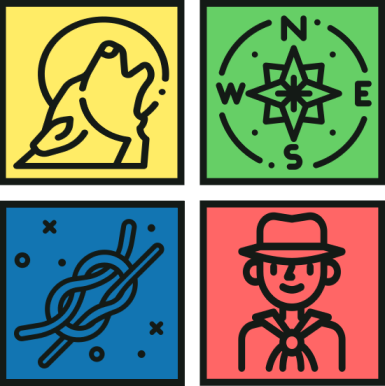
\includegraphics[width=0.45\textwidth]{logo.png}
    \caption{Logótipo da aplicação}
\end{figure}

Em termos funcionais, a aplicação concretiza diversos casos de uso, todos estes focados no ciclo de vida das actividades inerentes ao escutismo. O \gls{sitemap}, também este desenvolvido no decorrer da unidade curricular Desenvolvimento de Interfaces Aplicacionais, estabelece, de uma forma concisa e de simples interpretação, esses mesmos casos de uso. Analise-se o mesmo, na figura 2, adiante exposta:

\begin{figure}[H]
    \centering
    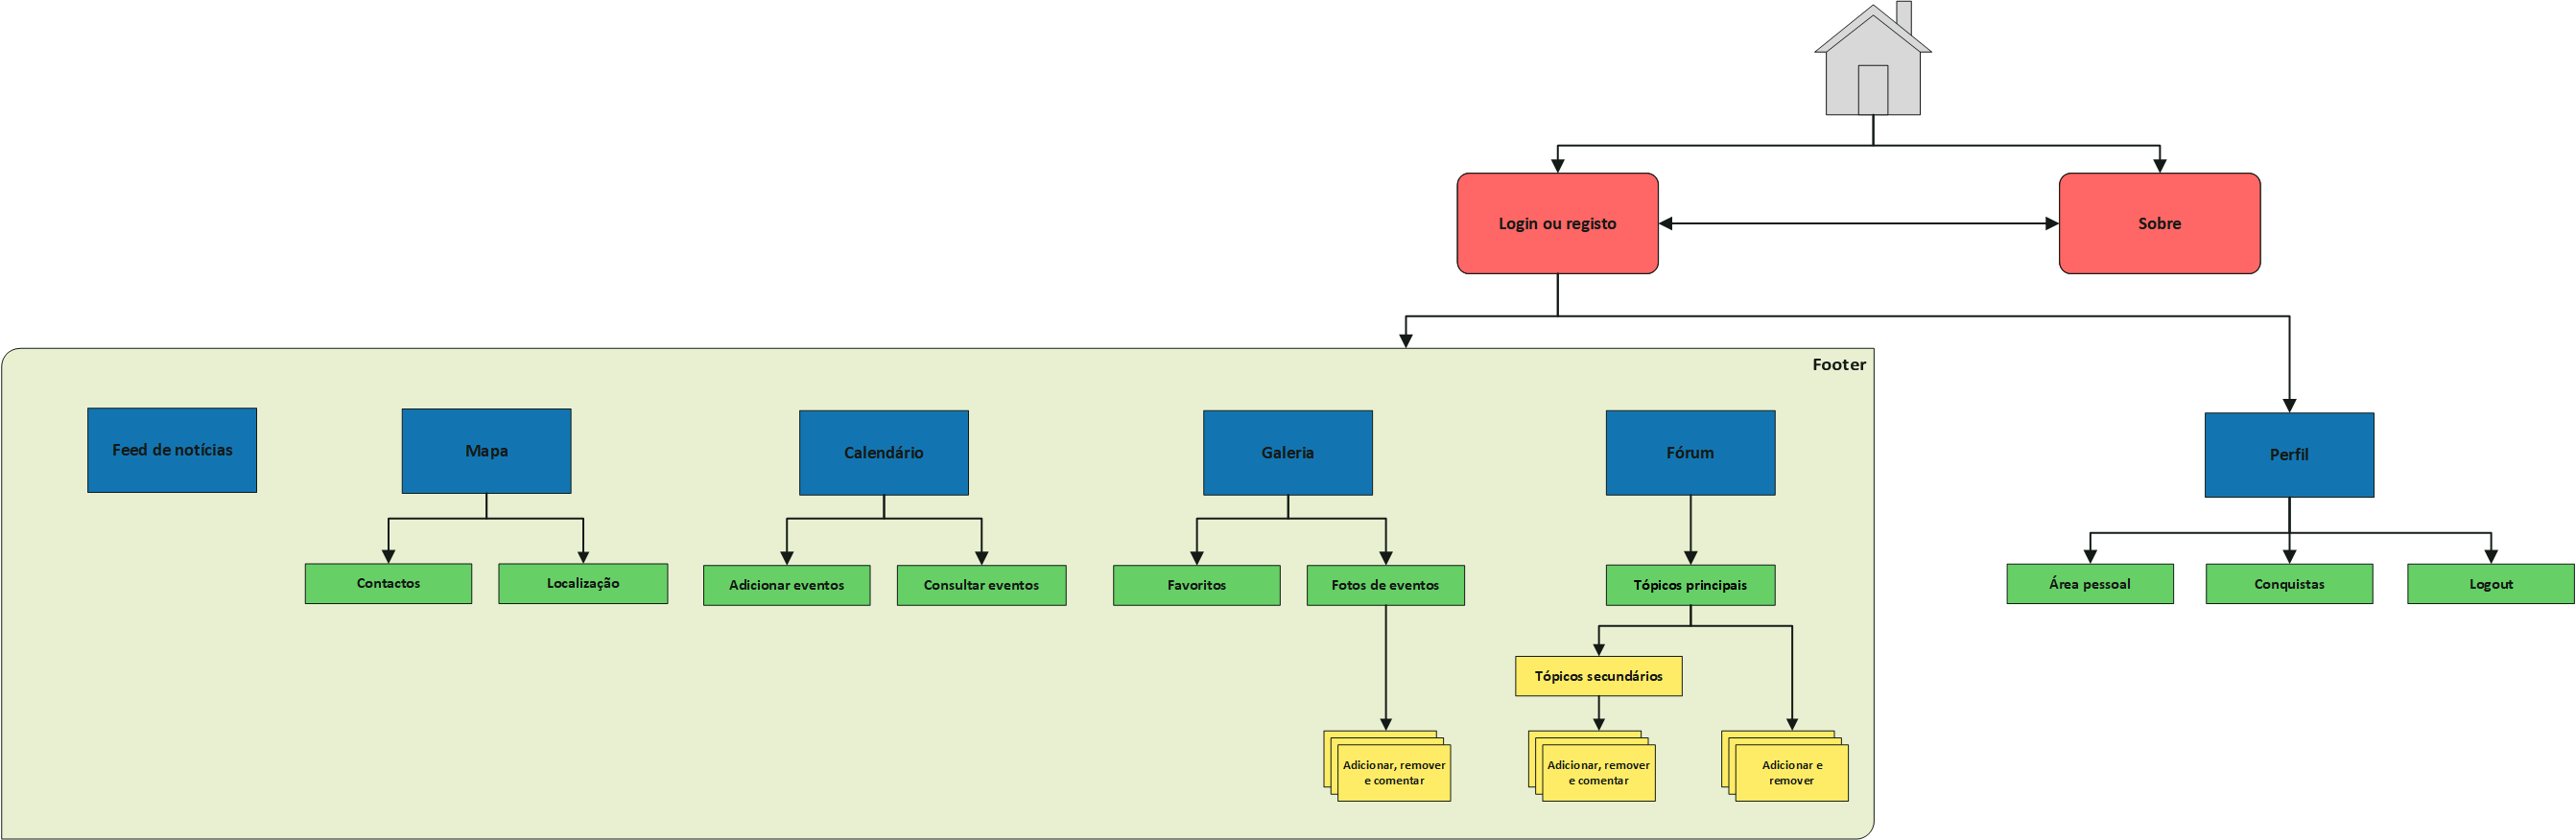
\includegraphics[width=1\textwidth]{sitemap.png}
    \caption{\gls{sitemap} da aplicação}
\end{figure}

Importa referir que, para efeitos do desenvolvimento do trabalho prático, o grupo de trabalho, juntamente com o professor Nuno Mendes, definiu alguns casos de uso como trabalho futuro. Isto porque não seria possível implementar todos os casos de uso em tempo útil. Dada a complexidade associada, optou-se pelos casos de uso associados ao fórum.

\clearpage

\section{Arquitectura da solução}

A solução desenvolvida baseia-se numa aplicação móvel, codificada na linguagem de programação \gls{kotlin} e linguagem de marcação \gls{xml}, que é compilada contra a \gls{api} nível 30 do sistema operativo \gls{android}. Além disso, recorre a variadas tecnologias na nuvem, que se caracterizam por modernas, flexíveis, extensíveis e escaláveis. Significativa parte das mesmas foram estudadas ou mencionadas no decorrer das aulas dedicadas à unidade curricular.

Numa perspectiva conceptual, é possível decompor a solução em diversos módulos distintos. Identifiquemos e avaliemos estes módulos, assim como respectivos componentes, através do diagrama presente na figura 3 adiante ilustrada:

\bigskip
\begin{figure}[H]
    \centering
    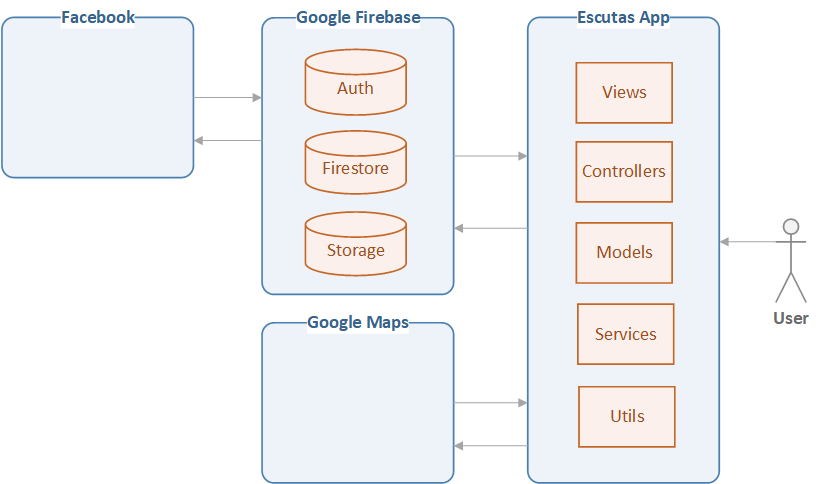
\includegraphics[width=1\textwidth]{architecture.png}
    \caption{Arquitectura da solução}
\end{figure}

Como é possível constatar, apesar do foco ser a aplicação móvel, a solução é efectivamente distribuída. Além disso, a aplicação móvel faz uso do padrão \gls{mvc}.

Tendo, como ponto de partida, o módulo que representa a aplicação móvel, segue-se uma breve descrição técnica de cada um dos componentes que compõem a solução.

\subsection{Serviços}

A camada de serviços da aplicação, é, na sua essência, responsável por abstrair os detalhes de comunicação da aplicação, com as respectivas dependências externas. De facto, é a camada de mais baixo nível da aplicação. 

O comportamento de cada um dos serviços é primeiramente definido por um interface, sendo depois o serviço concretamente implementado, com base no dito interface. Além disto, para cada um dos serviços, existe a respectiva excepção, que é devidamente despoletada, no momento em que um determinado erro ocorre. Examine-se, adiante, o propósito de cada um dos serviços:

\begin{itemize}
    \item \emph{FirebaseAuthService}: serviço responsável por convencionar os mecanismos de autenticação da aplicação, sendo que, para tal, usa serviços de autenticação do \gls{firebase}, que, por sua vez, comunicam com serviços do \gls{facebook}. Em síntese, o serviço possibilita a autenticação de utilizadores através de credenciais (e-mail e palavra-chave), conta \gls{google} ou conta \gls{facebook};
    
    \item \emph{FirebaseDatabaseService}: serviço capaz de comunicar com o repositório de dados da aplicação. Para tal, são implementadas operações \gls{crud} genéricas, independentes do modelo de dados. Conforme os requisitos estabelecidos no enunciado do trabalho prático, o repositório de dados utilizado é o \gls{firebase} Firestore. O mesmo segue o padrão não-relacional, que se caracteriza pela disponibilidade e escalabilidade;
    
    \item \emph{FirebaseStorageService}: serviço focado na comunicação com o repositório de \gls{blobs}, denominado de \gls{firebase} Storage. À semelhança do serviço previamente citado, implementa também operações \gls{crud} genéricas, agnósticas à tipologia dos \gls{blobs} em questão. É sobretudo usado para guardar imagens intrínsecas à aplicação. Embora este serviço não estivesse disposto como um requisito do trabalho prático, optou-se por o implementar, dada a sua manifesta utilidade. Compreenda-se, na figura 4 abaixo exposta, a estrutura do repositório de \gls{blobs}:
    
    % TODO: escrever sobre serviço SqliteDatabaseService.
\end{itemize}

\bigskip
\begin{figure}[H]
    \centering
    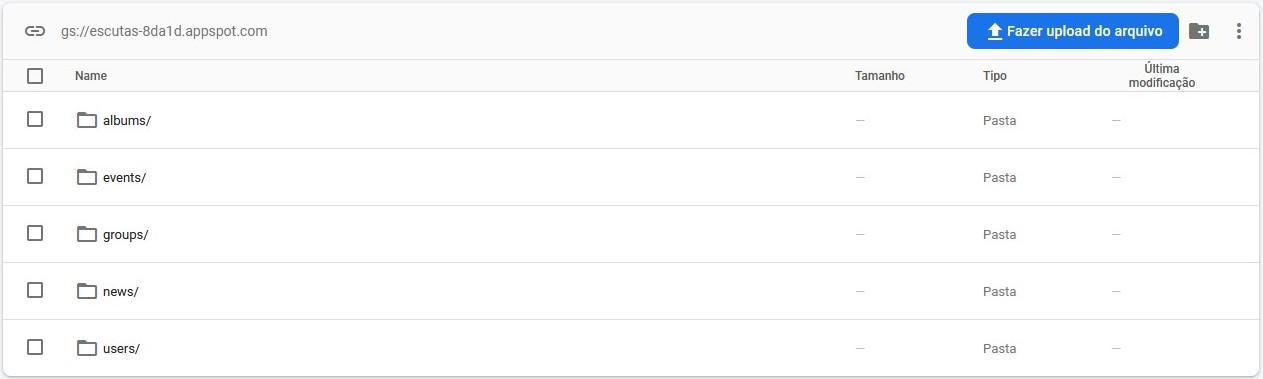
\includegraphics[width=1\textwidth]{storage.jpg}
    \caption{Estrutura do repositório de \gls{blobs}}
\end{figure}

\subsection{Modelos}

A aplicação define diversos modelos de dados. Os modelos de dados são depois instanciados e trocados entre as diferentes camadas da aplicação. Os mesmos apenas possuem estado e o seu desenho seguiu uma abordagem orientada ao domínio de negócio da aplicação. Veja-se os modelos de dados existentes:

\begin{itemize}
    \item \emph{Album}: como o nome indica, guarda um identificador, título e colecção de fotos. É expectável que o mesmo seja exibido na galeria da aplicação;
    
    \item \emph{Event}: compreende o nome, descrição, foto, data de inicio e data de término de um evento. Adicionalmente, define se este é ou não partilhável entre os utilizadores. Os eventos encontram-se dispostos no calendário da aplicação;
    
    \item \emph{Group}: integra o identificador, nome, descrição e coordenadas geográficas de um dado grupo de escutismo. Os marcadores do mapa da aplicação são desenhados com base nesta informação;
    
    \item \emph{News}: inclui o identificador, título, corpo e foto de uma qualquer notícia a ser apresentada no feed de notícias da aplicação;
    
    \item \emph{User}: engloba o identificador, email, nome, data de nascimento e grupo de escutismo de um determinado utilizador da aplicação.
\end{itemize}

\clearpage

\subsection{Controladores}

A camada de controladores da aplicação caracteriza-se por servir de intermediário entre a camada de serviços e a camada de vistas. Por consequência, contém expressiva parte da lógica de negócio da aplicação, uma vez que determina quando e de que forma os serviços são invocados e qual a informação que é disposta nas vistas. 

Para cada uma das vistas presentes na aplicação, existe o respectivo controlador. Todos estes controladores herdam de um controlador comum, apelidado de \emph{BaseController}, que inclui, como presumível, o estado e comportamento compartilhado. Por exemplo, os serviços de aplicação são instanciados no controlador comum, evitando assim que seja necessário instanciar os mesmos em cada um dos controladores derivados.

\subsection{Vistas}

A camada de vistas é a camada de mais alto nível da aplicação. Define-se como a camada de apresentação da solução, com a qual o utilizador interage directamente. 

No que diz respeito à estrutura da dita camada, existem elementos partilhados por considerável parte das vistas associadas, nomeadamente o cabeçalho e o rodapé. Estes são fundamentais para o funcionamento da aplicação e partilham da mesma responsabilidade: potenciar a usabilidade da aplicação e a experiência do utilizador.

O cabeçalho inclui, opcionalmente, um botão que permite o utilizador regressar para a vista anterior, o título da vista actual e a  imagem de perfil do utilizador. Ao pressionar a referida imagem de perfil, o utilizador é encaminhado para a sua área pessoal. Já o rodapé, compreende diversos botões, dispostos na horizontal, que possibilitam que o utilizador alterne entre as vistas que concretizam os principais casos de uso da aplicação, todos estes sujeitos a autenticação prévia. Para tal, a camada de vistas faz amplo uso de fragmentos, que são injectados entre o cabeçalho e o rodapé, através de uma vista base.

Complementarmente, a forma, disposição e dinamismo das vistas é construída com recurso a múltiplos ficheiros acessórios, que especificam cores, formas, vectores, fontes tipográficas e texto passível de ser localizado.

Considere-se, de seguida, uma explicação funcional, para cada uma das vistas presentes na aplicação, acompanhadas de figuras que ilustram a sua aparência:

\begin{itemize}
    \item \emph{Splash}: vista relativamente simples, na medida em que apenas exibe o logótipo da aplicação. A mesma é apresentada no arranque da aplicação, por um período de tempo programaticamente definido. Observe-se a figura 5 abaixo indicada:
    
    \bigskip
    \begin{figure}[H]
        \centering
        
\includegraphics[width=0.5\textwidth]{view-splash.png}
        \caption{Vista Splash}
    \end{figure}
    
    \item \emph{Login}: vista apresentada após o arranque supra citado. Na mesma, é possível realizar a autenticação através de credenciais, conta \gls{facebook} ou conta \gls{google}. Além disto, é também possível seguir para as vistas responsáveis pelo registo na aplicação ou recuperação de credenciais. Por último, é ainda exequível prosseguir para uma vista que expõe informação contextual sobre a aplicação. Averigúe-se a aparência da mencionada vista, através da figura 6, que se segue:
    
    \bigskip
    \begin{figure}[H]
        \centering
        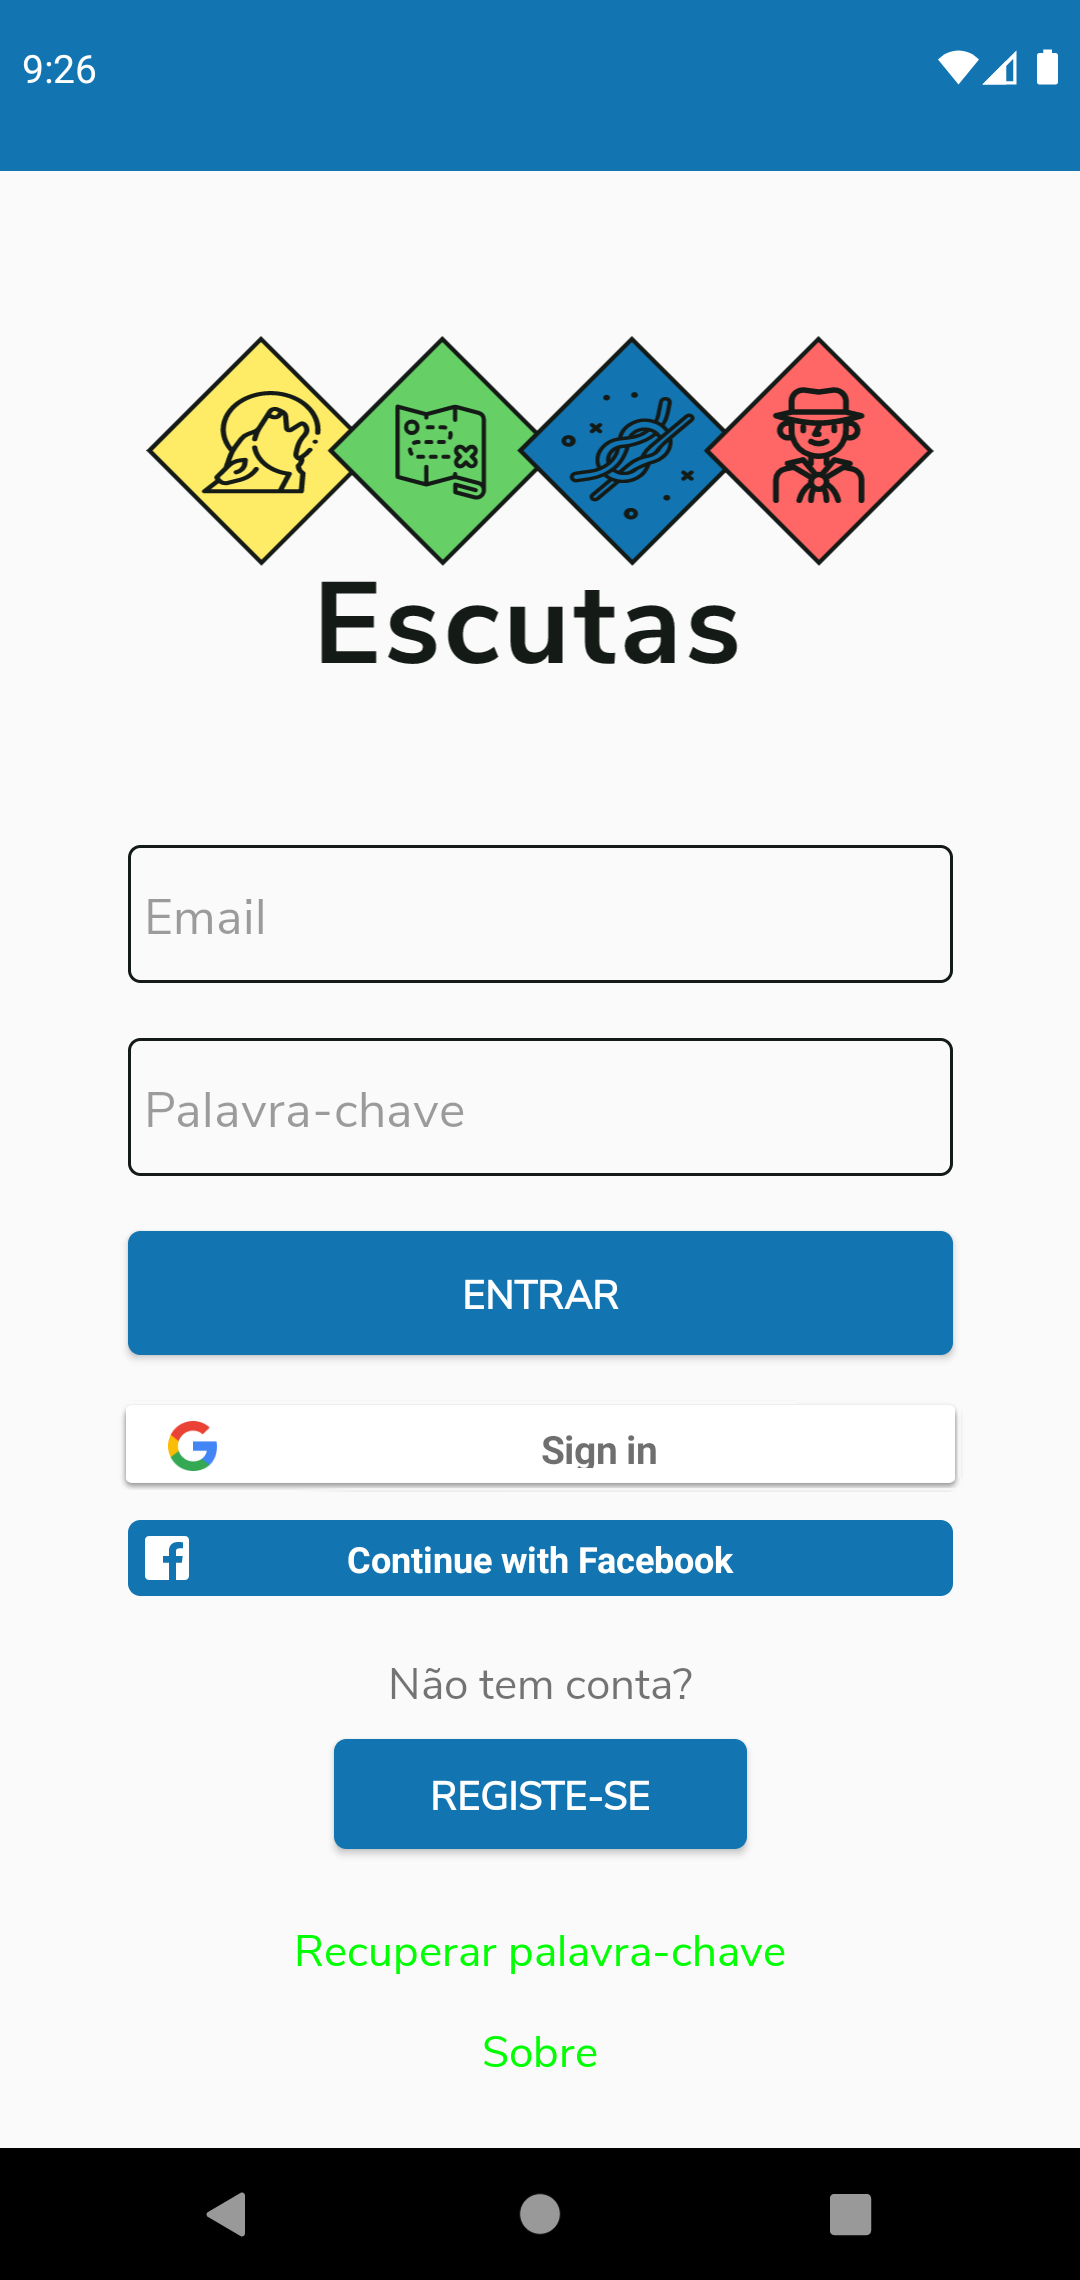
\includegraphics[width=0.5\textwidth]{view-login.png}
        \caption{Vista Login}
    \end{figure}
    
    \item \emph{Register}: como o nome sugere, é a vista responsável pelo registo na aplicação, através de credenciais convencionais - email e palavra-chave. No caso de um utilizador optar pelas restantes formas de autenticação, na primeira vez que a realizar, será apresentada uma vista semelhante, contudo adaptada ao respectivo mecanismo de autenticação. Com vista a promover clareza, para efeitos de demonstração, é apresentada, através das figuras 7 e 8 infra mencionadas, a vista de registo através de credenciais convencionais. Já a vista de registo alternativa, poderá ser  convenientemente consultada no código fonte da aplicação.
    
    \bigskip
    \begin{figure}[H]
        \centering
        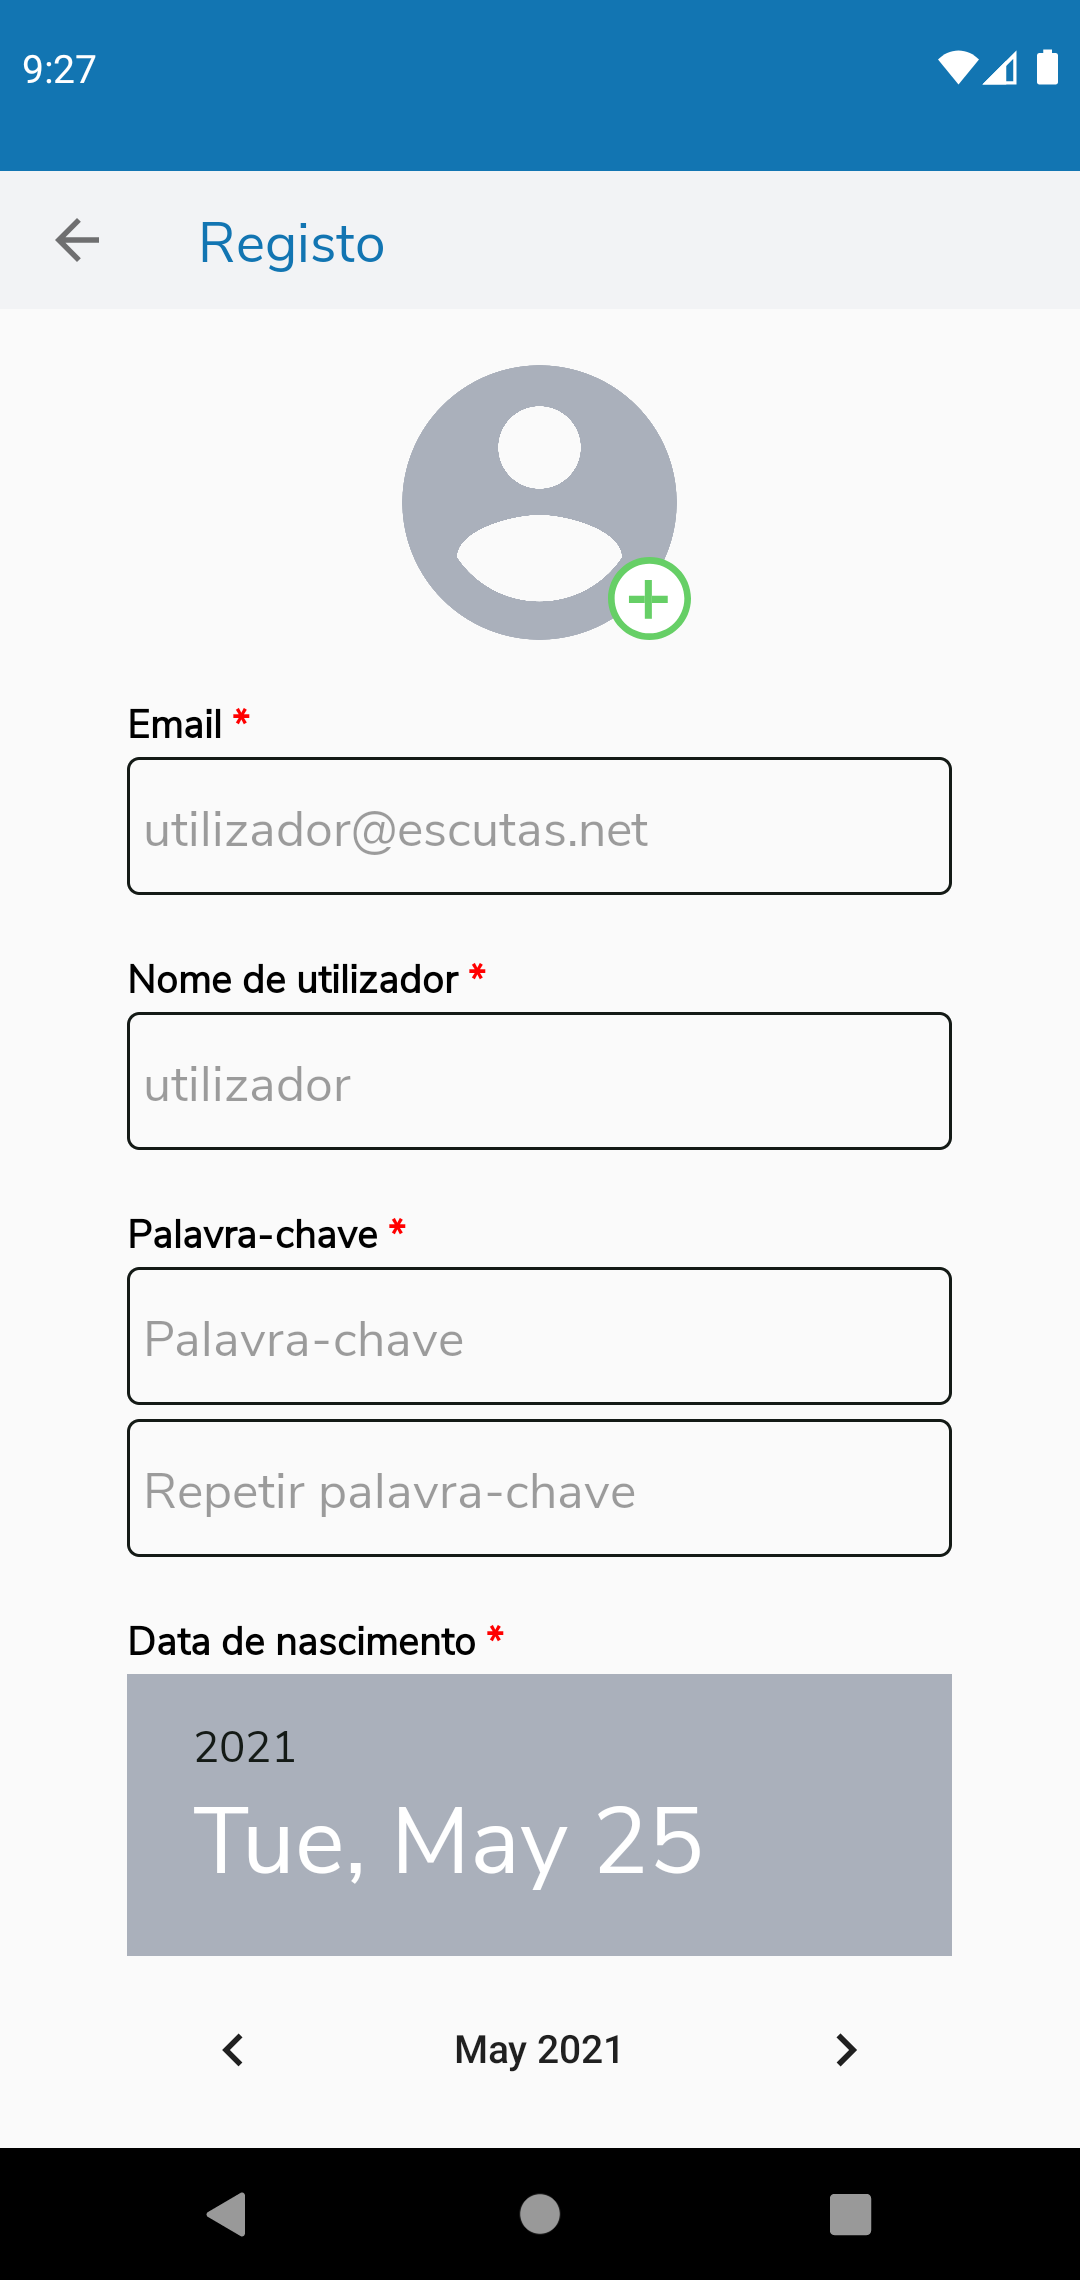
\includegraphics[width=0.34\textwidth]{view-register-1.png}
        \caption{Vista Register}
    \end{figure}
    
    \bigskip
    \begin{figure}[H]
        \centering
        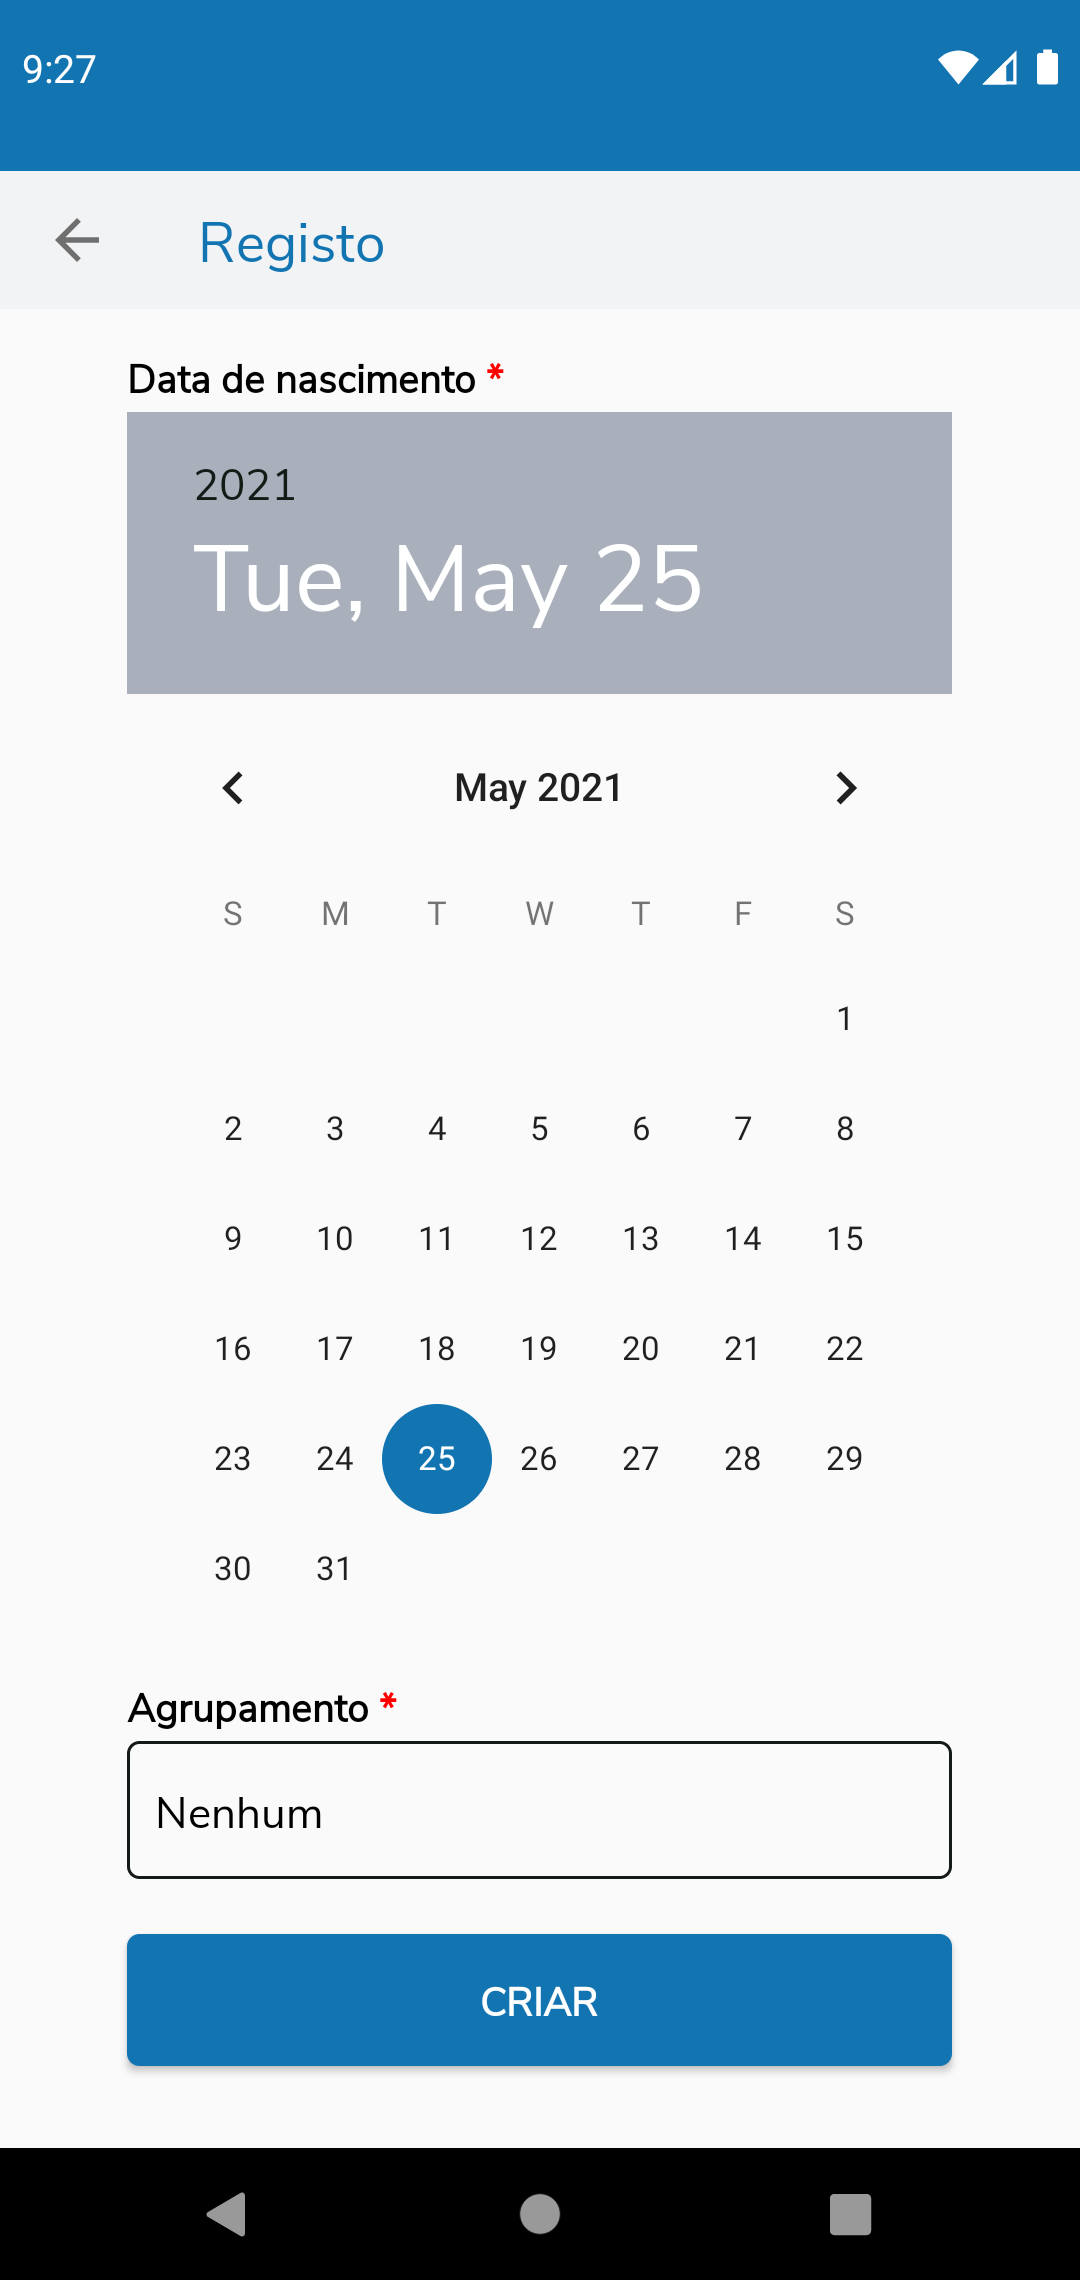
\includegraphics[width=0.34\textwidth]{view-register-2.png}
        \caption{Vista Register (continuação)}
    \end{figure}
    
    \item \emph{Recover}: se por ventura, um qualquer utilizador, registado através de credenciais convencionais, perder a sua palavra-chave, terá que a conseguir recuperar. A presente vista proporciona esse mesmo caso de uso. Verifique-se a figura 9:
    
    \bigskip
    \begin{figure}[H]
        \centering
        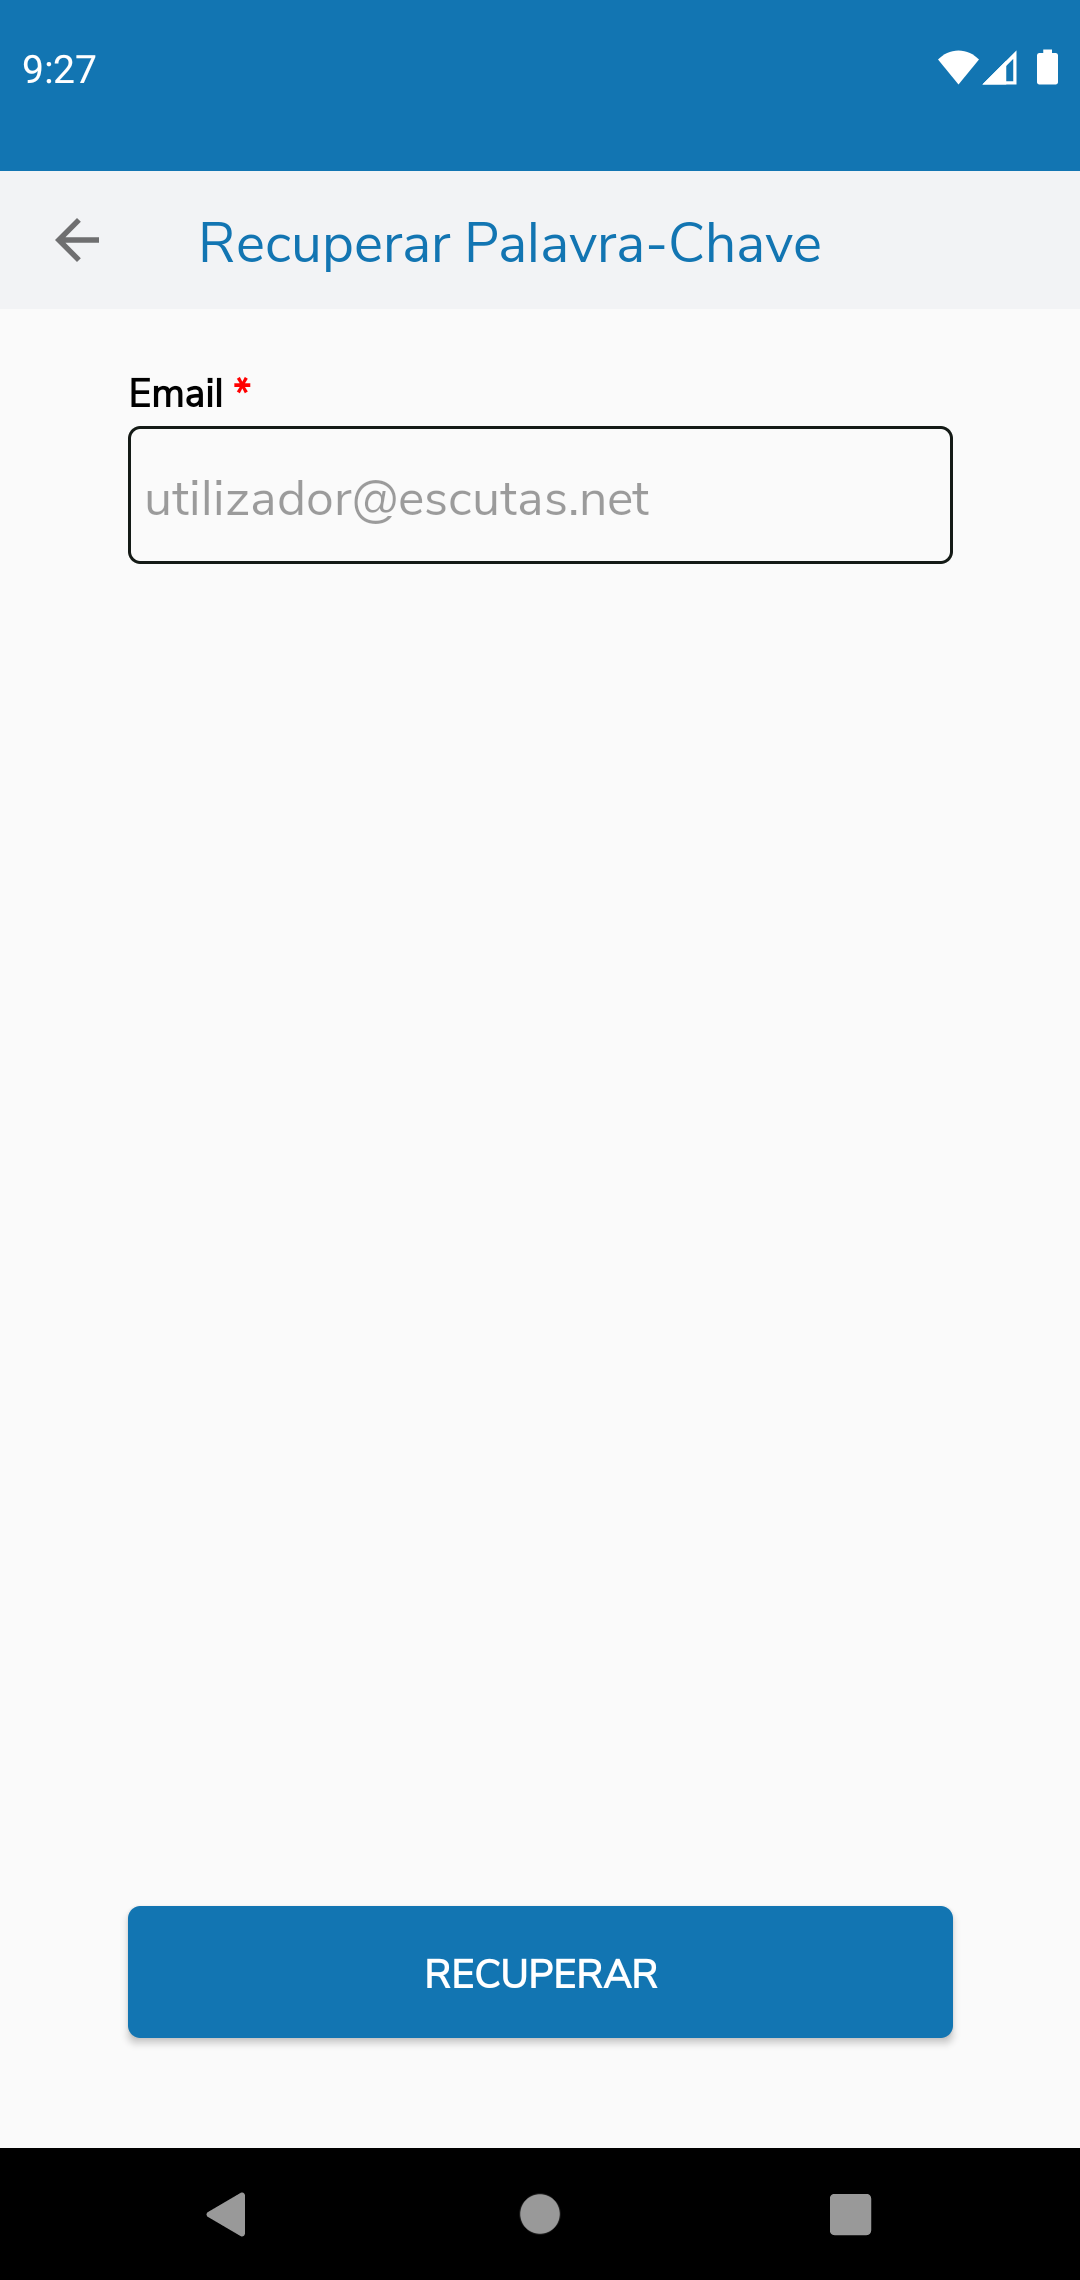
\includegraphics[width=0.5\textwidth]{view-recover.png}
        \caption{Vista Recover}
    \end{figure}
    
    \item \emph{About}: vista estática, e consequentemente simples, que abrange informação contextual sobre a aplicação. Nesta, está exposto o enquadramento da aplicação e o grupo de trabalho que desenvolveu a mesma, aliado aos respectivos meios de contacto. Confira-se a referida vista, por meio da figura 10, abaixo ilustrada:
    
    \bigskip
    \begin{figure}[H]
        \centering
        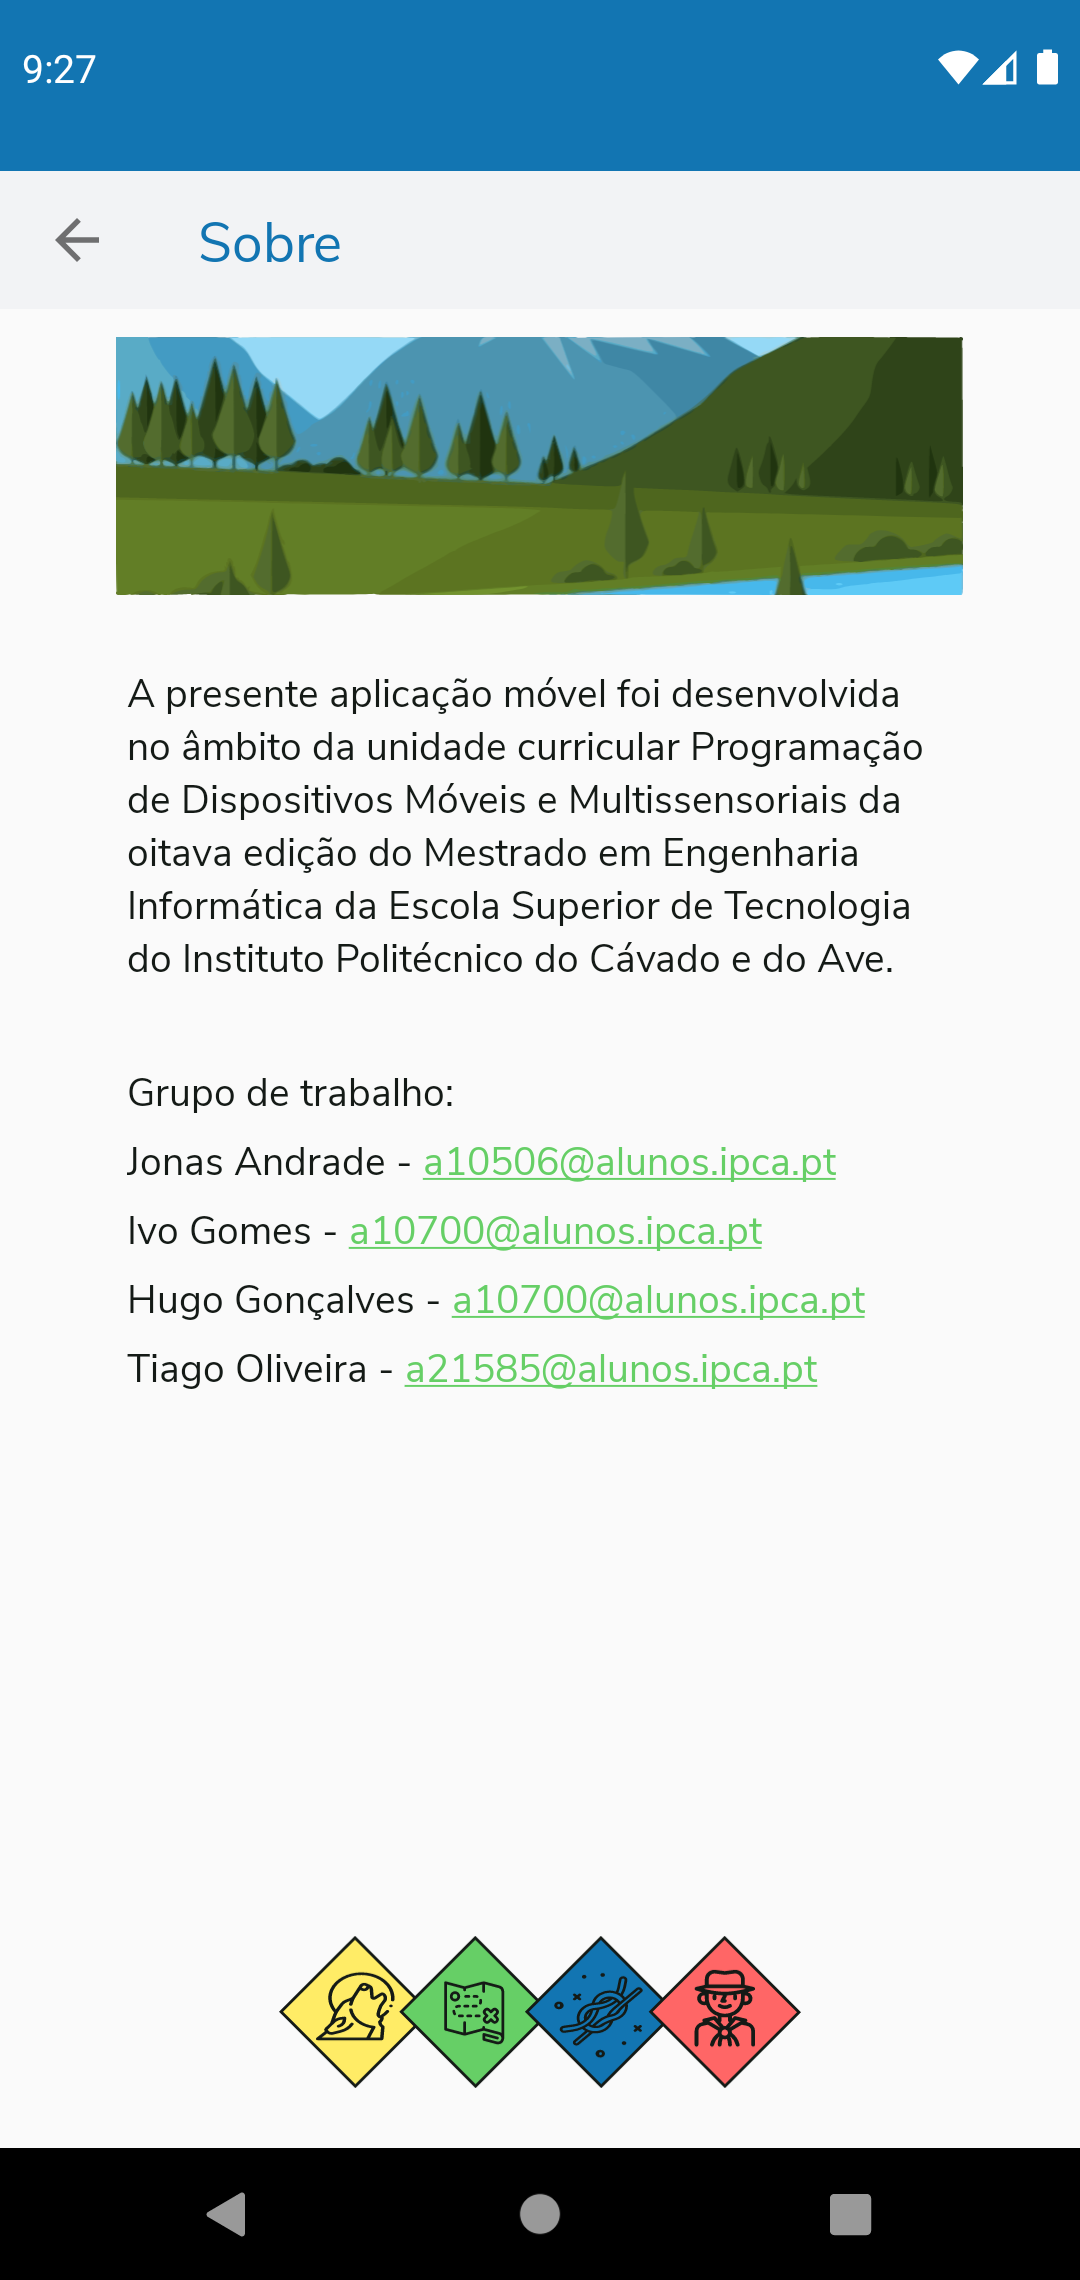
\includegraphics[width=0.5\textwidth]{view-about.png}
        \caption{Vista About}
    \end{figure}
    
    \item \emph{Profile}: vista que materializa a área pessoal do utilizador autenticado na aplicação. Esta é também relativamente descomplicada, na medida em que somente exibe os detalhes do respectivo utilizador e consente que este termine, graciosamente, a sessão na aplicação. Veja-se a referida vista na figura 11 seguidamente evidenciada:
    
    \bigskip
    \begin{figure}[H]
        \centering
        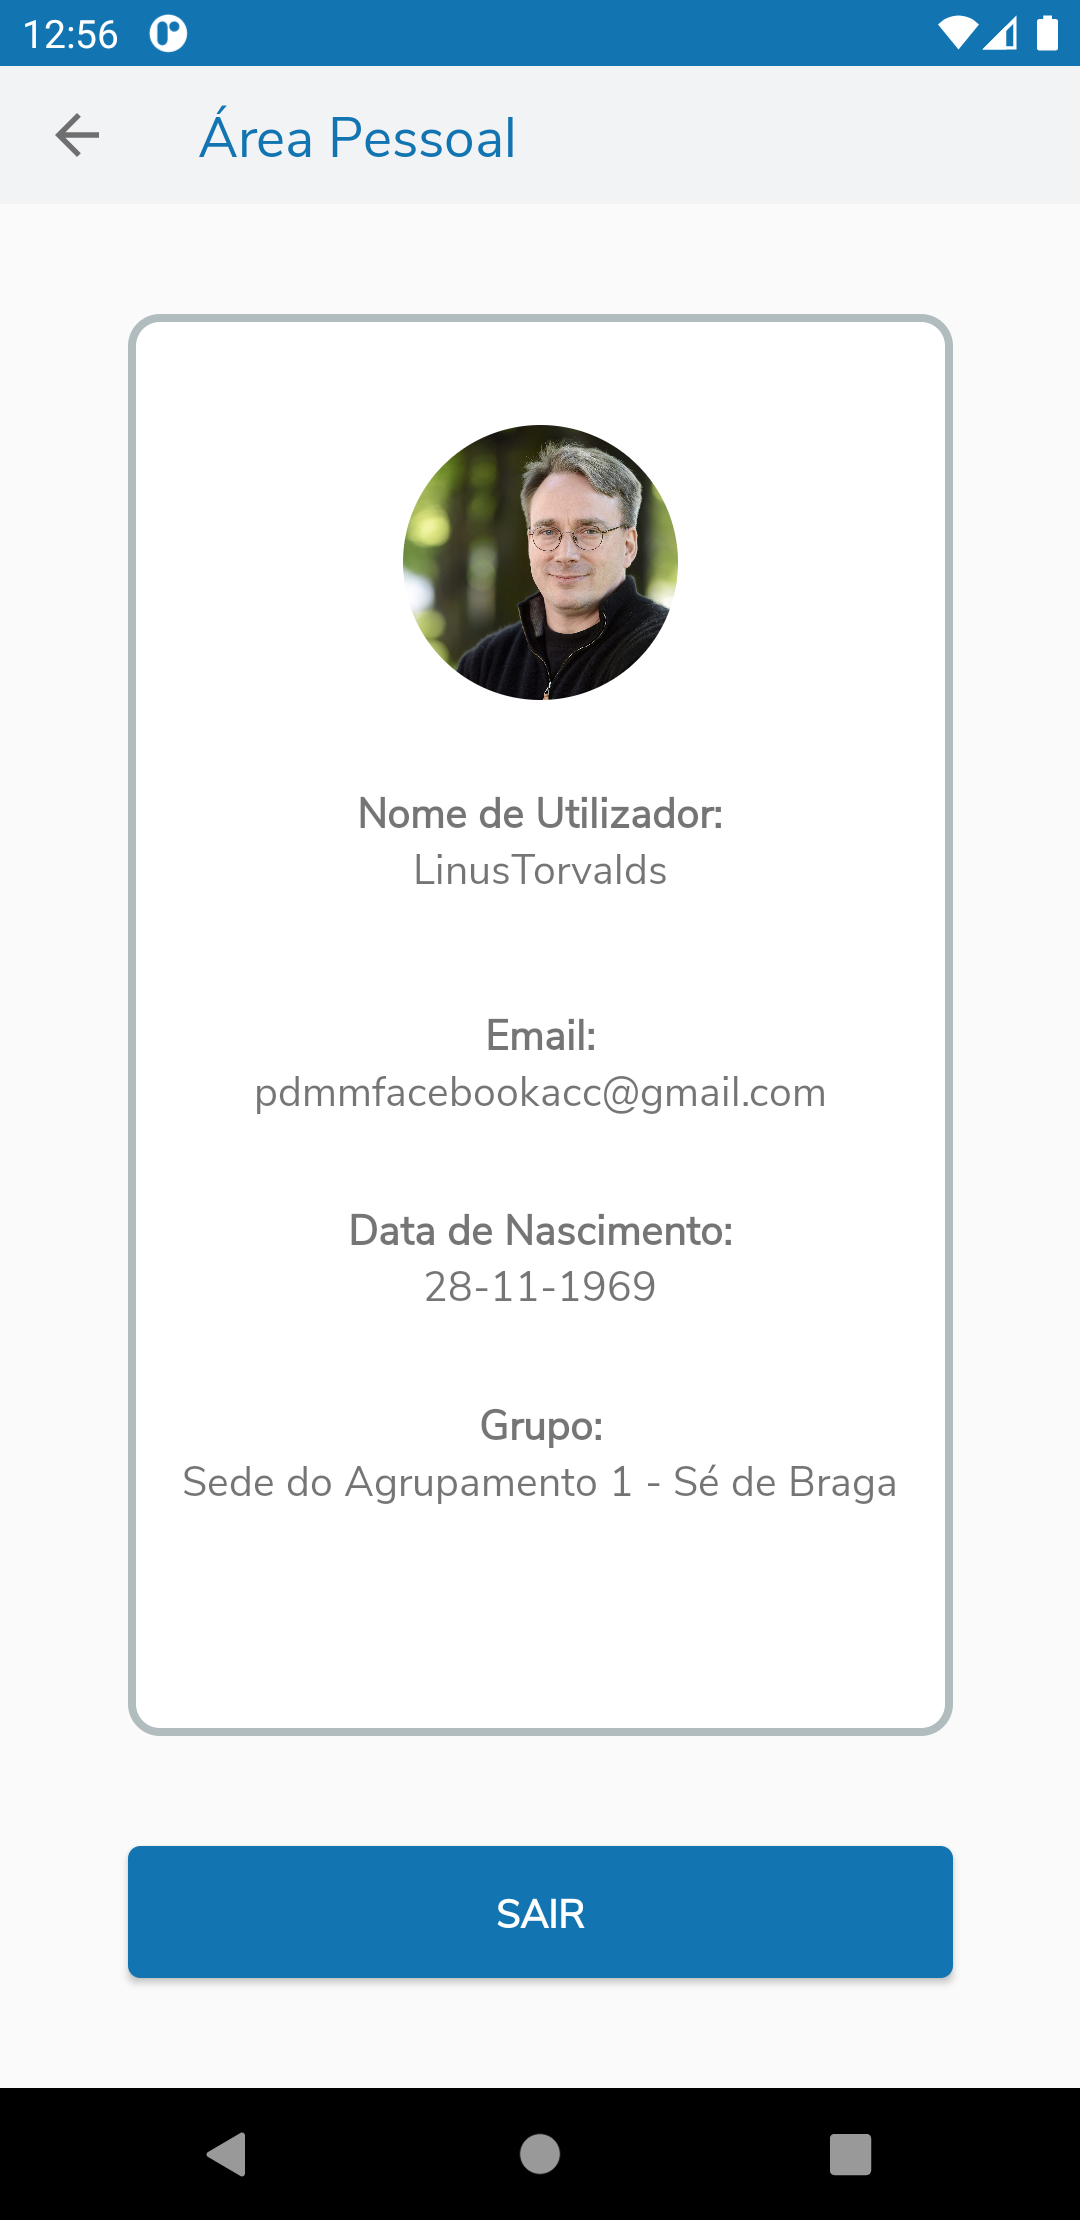
\includegraphics[width=0.5\textwidth]{view-profile.png}
        \caption{Vista Profile}
    \end{figure}
    
    \item \emph{Map}: vista encarregue de apresentar, através de um mapa interactivo, os grupos de escutismo que se encontram nas proximidades do utilizador da aplicação. Para tal, recorre à \gls{api} do \gls{maps} e a mecanismos de localização do sistema operativo \gls{android}. Por sua vez, o referido sistema operativo utiliza o sensor \gls{gps} do dispositivo. Seguindo as boas práticas de desenvolvimento \gls{android}, as permissões de localização são meramente requeridas no momento em que se tornam indispensáveis. Perceba-se a vista na figura 12 que se segue:
    
    \bigskip
    \begin{figure}[H]
        \centering
        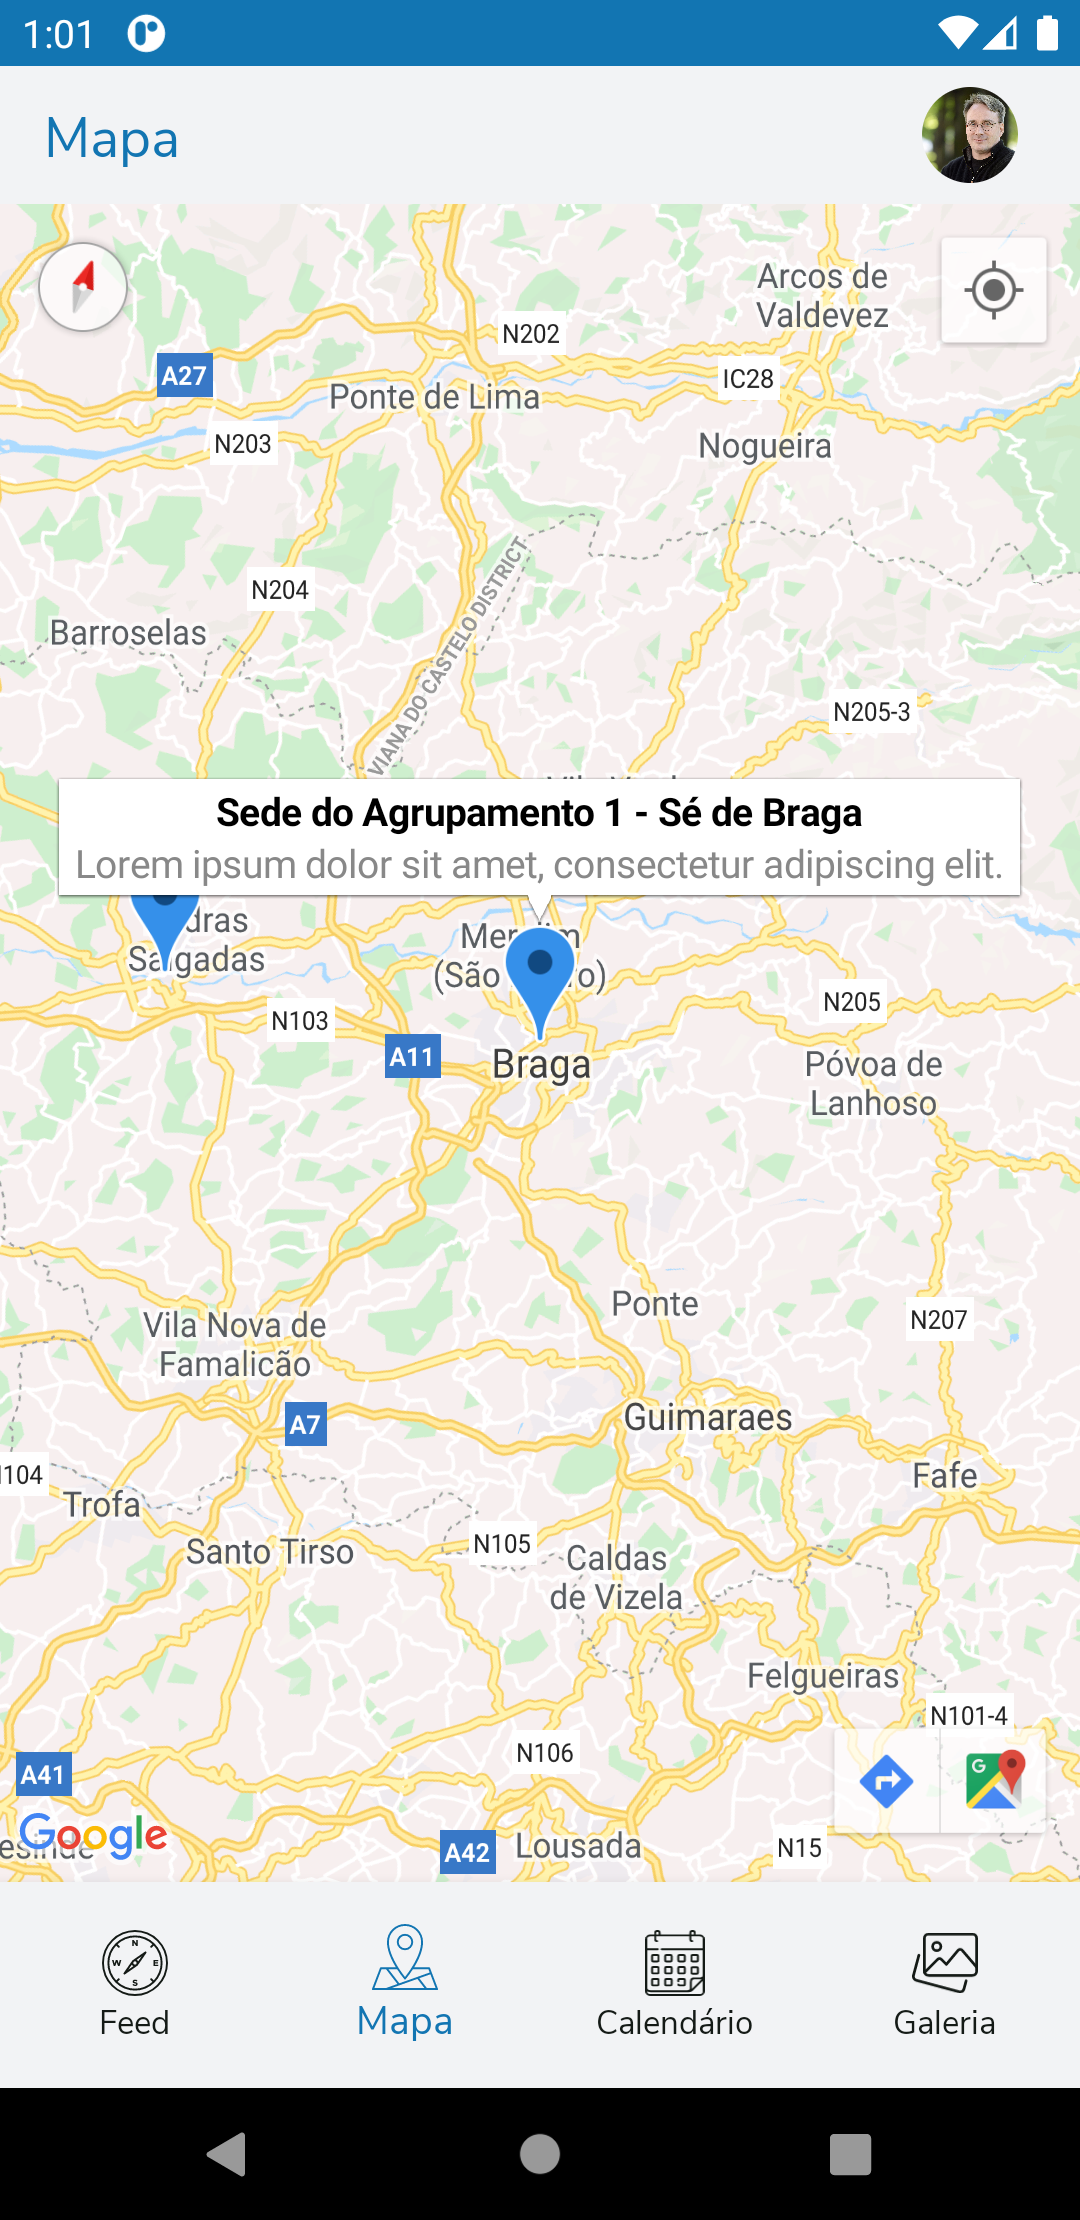
\includegraphics[width=0.5\textwidth]{view-map.png}
        \caption{Vista Map}
    \end{figure}

    % TODO: escrever sobre vista de notícias, galeria e calendário.
\end{itemize}

\clearpage

\subsection{Utilitários}

Os utilitários são componentes genéricos e transversais, que podem ser utilizados por uma qualquer camada da aplicação, e que visam promover a reutilização de código. Os mesmos não têm estado, encontram-se organizados por tipo de dados e incluem exclusivamente métodos estáticos, que realizam tarefas pequenas e repetidas. Considere-se uma síntese de cada um dos utilitários:

\begin{itemize}
    \item \emph{StringUtils}: utilitário que guarda métodos intrínsecos ao tipo de dados \textit{string}. Por exemplo, um métodos de extensão contido neste utilitário, valida se uma determinada \textit{string} segue o padrão de um endereço de email, através do uso de expressões regulares; 
    
    \item \emph{DateUtils}: utilitário que armazena métodos inerentes ao tipo de dados \textit{Date}. Exemplificando, neste utilitário, existe um método, que recebe como argumentos, um dia, mês e ano - no tipo de dados \textit{int}. Devolve, consequentemente, a respectiva data - no tipo de dados \textit{Date}.
\end{itemize}

\clearpage

\section{Metodologia de desenvolvimento}

A metodologia de desenvolvimento da aplicação focou-se em três vectores de acção: versionamento, planeamento e boas práticas. As sub-secções que se seguem abordam, para cada um dos vectores de acção supra citados, os tópicos considerados relevantes.

\subsection{Versionamento}

As operações de versionamento da aplicação, recorrem ao sistema de controlo de versões \gls{git}, cujo repositório encontra-se alojado na plataforma \gls{github}. Os elementos do grupo de trabalho têm o devido acesso ao repositório e podem, consequentemente, contribuir para o mesmo, conforme a organização e regras estipuladas. Começando pela organização do repositório, o mesmo é composto por diversos ramos, que servem diferentes propósitos. Considere-se cada um deles:

\begin{itemize}
    \item \emph{dev}: ramo de desenvolvimento ativo, para onde as contribuições provenientes dos ramos de cada elemento do grupo de trabalho, são fundidas. Dada a sua natureza, os binários resultantes da compilação do código fonte do presente ramo poderão encontrar-se num estado instável;
    
    \item \emph{qa}: ramo exclusivamente dedicado a testes, com vista a assegurar a qualidade e estabilidade da aplicação desenvolvida. Ao contrário do ramo anteriormente referido, o presente ramo não acolhe contribuições individuais, sendo que é simplesmente sincronizado com o ramo anterior, em momentos considerado oportunos pelo grupo de trabalho;
    
    \item \emph{main}: quando, depois dos testes realizados na linha previamente citada, uma determinada versão da aplicação é considerada plenamente funcional e estável, o seu conteúdo é sincronizada com a presente linha. A partir desta, são geradas \textit{releases} com binários aptos para produção. A título de exemplo, os binários submetidos no trabalho prático, são provenientes da presente linha.
\end{itemize}

No que diz respeito a regras, uma determinada contribuição de um elemento do grupo de trabalho, é necessariamente realizada através de um \textit{pull request}. Neste, o elemento terá que responder a uma série de questões sobre o conteúdo e finalidade da sua contribuição, previamente fixadas num \textit{pull request template}. 

Após a submissão do \textit{pull request}, o mesmo é eventualmente revisto pelos restantes elementos do grupo de trabalho. Mediante a revisão, o grupo de trabalho poderá aceitar, rejeitar ou requerer modificações à contribuição. Assim que a contribuição for aceite por, pelo menos, dois elementos do grupo de trabalho, o autor da contribuição poderá fundir a sua contribuição com a linha alvo. Observe-se os detalhes de um \textit{pull request}, realizado durante o decorrer do desenvolvimento do trabalho prático, na figura 13, adiante ilustrada:

\bigskip
\begin{figure}[H]
    \centering
    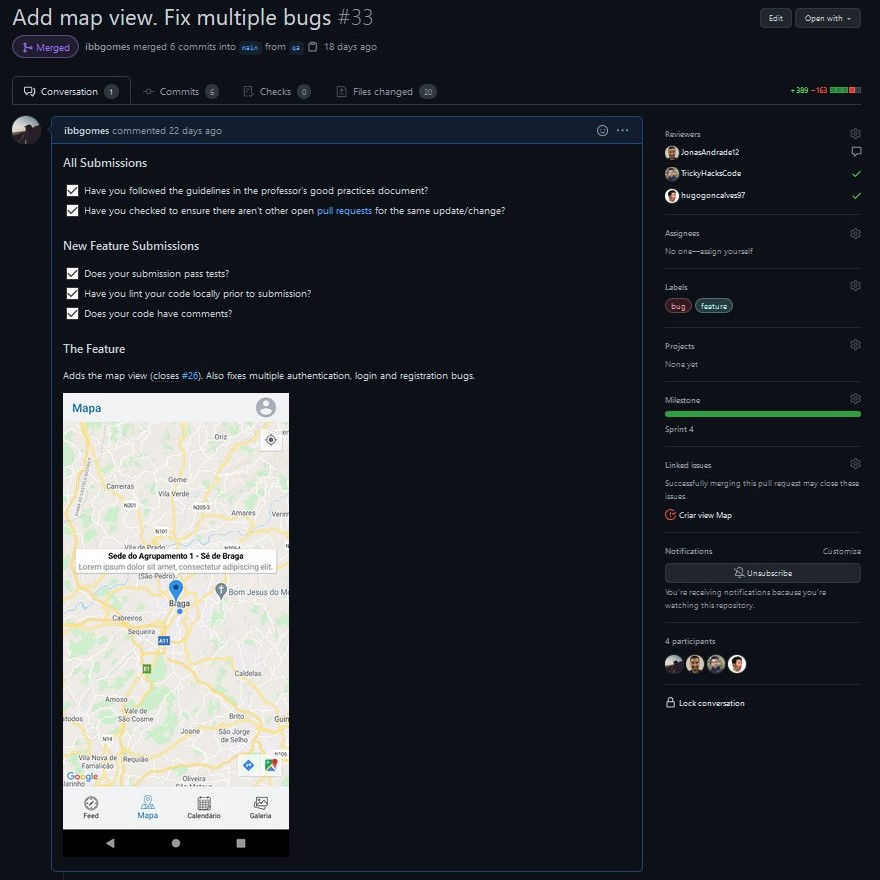
\includegraphics[width=1\textwidth]{pull-request.png.jpg}
    \caption{Exemplo de um \textit{pull request}}
\end{figure}

\subsection{Planeamento}

O desenvolvimento da aplicação foi planeado e gerido com recurso a metodologias de desenvolvimento ágeis, nomeadamente a \gls{framework} Scrum, sendo que cada \gls{sprint} teve a duração de uma semana, decorrida entre aulas dedicadas à unidade curricular.

Com vista a auxiliar as tarefas de planeamento e gestão associadas ao processo de desenvolvimento da aplicação, recorreu-se às ferramentas de gestão de projecto da plataforma \gls{github}. Primeiramente, começou-se por especificar Sprints até à data estabelecida para a entrega do trabalho prático, em forma de \textit{milestones}. Veja-se algumas destas Sprints, através da figura 14, seguidamente disposta:

\bigskip
\begin{figure}[H]
    \centering
    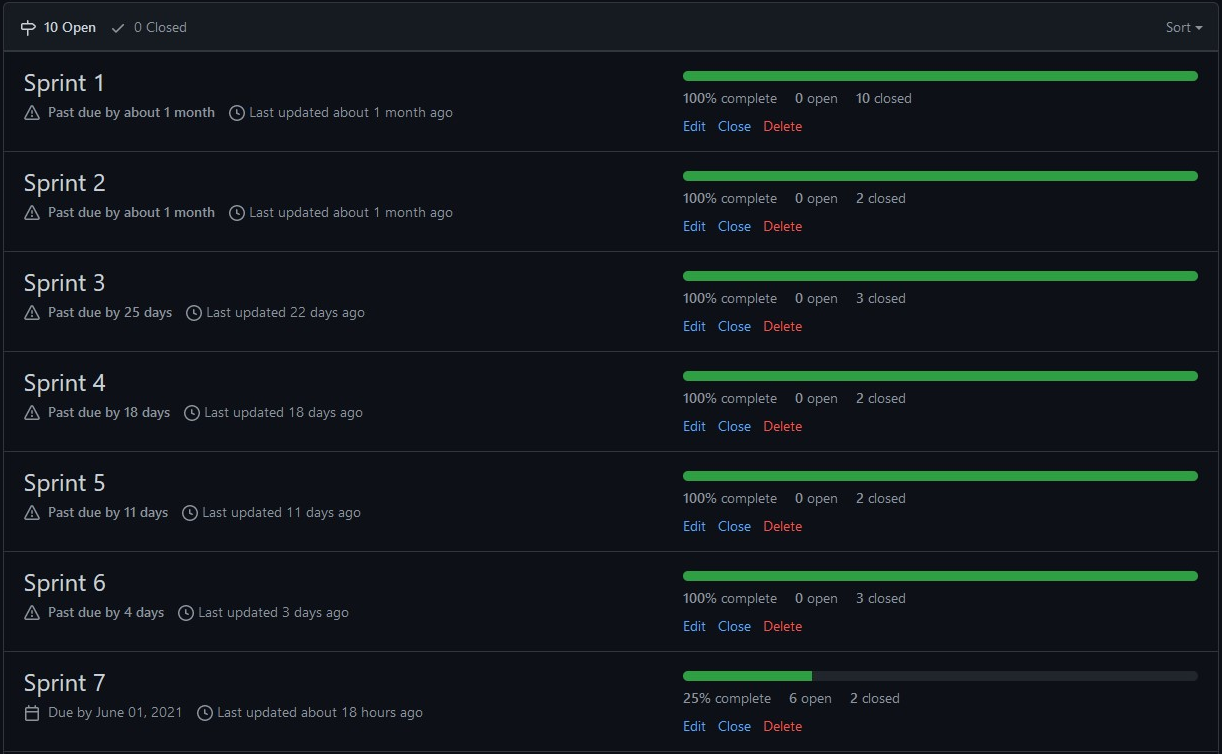
\includegraphics[width=1\textwidth]{sprints.png}
    \caption{Sprints do projecto}
\end{figure}

Em cada uma das aulas da unidade curricular, onde o grupo de trabalho estava presencialmente ou remotamente reunido, procedeu-se ao planeamento da \gls{sprint} seguinte, através da alocação de tarefas provenientes do \gls{backlog} do projecto, regularmente mantido sob a forma de \textit{issues}. Analise-se, em baixo, a figura 15, que demonstra o \gls{backlog} do projecto num dado instante:

\bigskip
\begin{figure}[H]
    \centering
    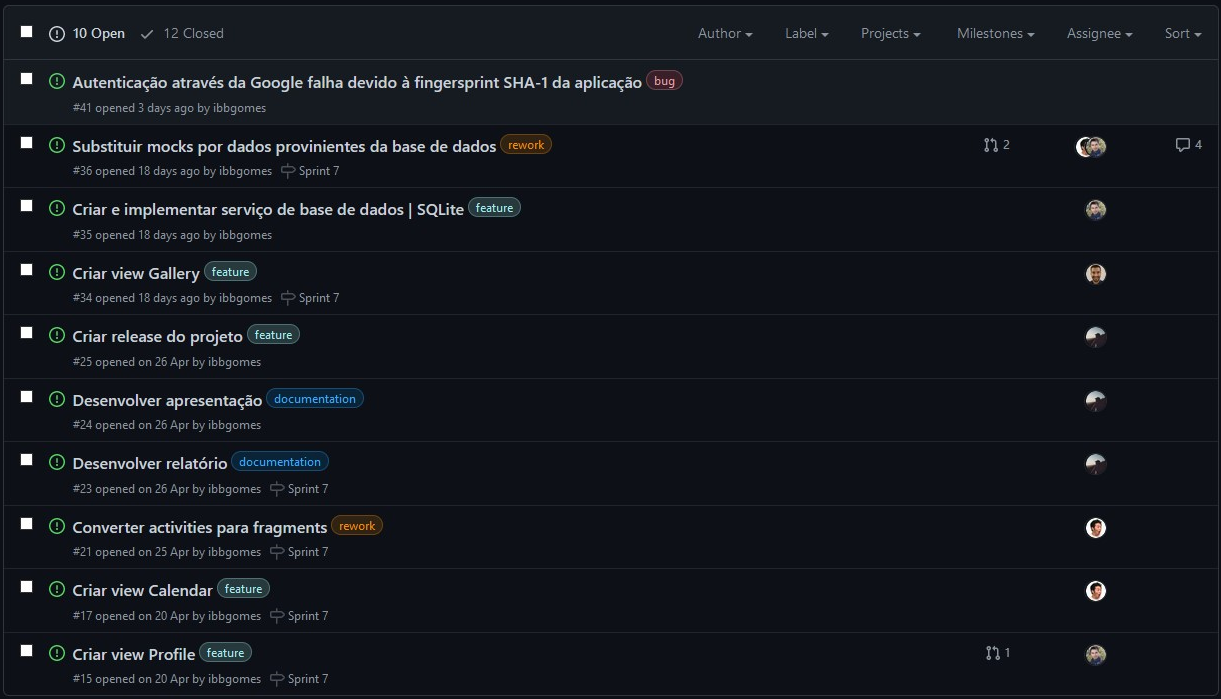
\includegraphics[width=1\textwidth]{backlog.png}
    \caption{Backlog do projecto}
\end{figure}

Como é possível constatar na figura anteriormente citada, as tarefas assumem variadas tipologias. Para concretizar tal coisa, foram definidas \textit{labels}, através de cores sugestivas, que refletem a positividade da tarefa no contexto do desenvolvimento do projecto. Faça-se uma breve descrição de cada uma delas:

\begin{itemize}
    \item \emph{Feature}: representa uma tarefa que diz respeito ao desenvolvimento de uma qualquer nova funcionalidade na aplicação;
    
    \item \emph{Documentation}: retrata uma tarefa de documentação. Por exemplo, a escrita do presente documento, foi definida como tarefa de documentação;
    
    \item \emph{Rework}: corresponde a uma tarefa que implica a reestruturação de uma dada funcionalidade existente na aplicação;
    
    \item \emph{Bug}: refere-se a uma tarefa que incide sobre a resolução de um determinado erro identificado na aplicação.
\end{itemize}

\clearpage

\subsection{Boas práticas}

No decorrer da construção da aplicação, fez-se por seguir ou implementar aquilo que são transversalmente reconhecidas como boas práticas de desenvolvimento de software. Examine-se algumas das práticas empregues:

\begin{enumerate}
    \item Dado que a aplicação foi desenvolvida através do paradigma de programação orientada a objectos, fez-se por cumprir os princípios \gls{solid}. Adicionalmente, com vista a promover a manutibilidade e simplicidade do código fonte, seguiu-se também os princípios \gls{dry} e \gls{kiss};
    
    \item De modo a detectar erros e garantir a uniformidade do código fonte, fez-se uso de um \gls{linter}, direccionado à linguagem de programação \gls{kotlin}, que se encontra convenientemente integrado com o sistema de automação de compilação da aplicação. O mesmo é apelidado de \textit{ktLint}, é activamente desenvolvido pelo \gls{pinterest} e encontra-se ao abrigo de uma licença de código aberto;
    
    \item O código fonte da aplicação, quando compilado para ambientes de produção, gera binários que se encontram adequadamente compactados, optimizados e ofuscados. Para tal, são utilizadas as opções de compilação \textit{minifyEnabled} e \textit{shrinkResources}.
\end{enumerate}

\clearpage

\section{Desafios de implementação}

O principal desafio de implementação da aplicação, foi o facto de nenhum elemento do grupo de trabalho, ter  conhecimento ou experiência prévia no desenvolvimento de aplicações móveis. Como expectável, este facto traduziu-se numa velocidade de implementação inicialmente reduzida, que foi progressivamente aumentando, à medida que o grupo de trabalho adquiria conhecimento, experiência e agilidade na plataforma \gls{android}, \gls{firebase} e tecnologias associadas.

Existiram ainda alguns contratempos na implementação de rotinas assíncronas através da linguagem de programação \gls{kotlin}. Não obstante, estes foram trivialmente ultrapassados, através de espírito de entreajuda e auxílio do professor.

% TODO: escrever sobre problema de autenticação através de conta Google.

\chapter{Conclusão}

Terminado o trabalho prático e considerando a natureza empírica do mesmo, cremos que o trabalho desenvolvido foi essencial para a consolidação dos conhecimentos transmitidos pelo professor no decorrer das aulas dedicadas às temáticas abordadas. Acreditamos também que o desenvolvimento deste permitiu amadurecer as nossas competências técnicas na área de programação móvel - nomeadamente no que diz respeito ao ecossistema \gls{android}. Tivemos ainda oportunidade de explorar o referido ecossistema através de ferramentas até então não empregues, como foi o caso do \gls{firebase} e \gls{maps}, o que foi uma experiência altamente gratificante.

Relativamente ao trabalho desenvolvido, julgamos que este cumpre competentemente os requisitos mencionados no desafio que nos foi lançado pelo professor. Gostaríamos de ter desenvolvido um trabalho mais aprofundado - particularmente na implementação de pequenos pormenores funcionais que tornariam a aplicação mais rica - contudo, a carga de trabalho característica de uma pós-graduação, aliada às nossas obrigações profissionais, limitou o tempo passível de ser despendido a trabalhar para cada uma das unidades curriculares.

\bibliography{refs}
\bibliographystyle{ieeetr}
\nocite{*}

\end{document}